
\chapter{Introducción}

% --------------------------------------------------------------------------------------------------------------------------

\section{Descripción del problema}

La antropología es la ciencia que estudia la humanidad en todas sus dimensiones: biológica, cultural, 
lingüística o arqueológica \cite{AAA2022AnthropologyDefinition}, a lo largo del tiempo y en distintas partes 
del mundo. La antropología biológica o física se centra en el estudio de la anatomía, el crecimiento, la 
adaptación y la evolución del cuerpo humano \cite{nawrocki2006}. 

Dentro de este campo, la \textbf{antropología forense (AF)} es el subcampo especializado que aplica métodos y 
técnicas antropológicas para resolver cuestiones médico-legales \cite{nawrocki2006}, empleando conocimientos 
de antropología física, aunque a veces también de la arqueología, para la correcta recuperación y análisis de 
la evidencia forense.

Tradicionalmente, los antropólogos forenses han tenido cinco principales objetivos en su trabajo 
\cite{byers2023}:

\begin{enumerate}

    \item Determinar el \textbf{perfil biológico} de un individuo (es decir, sexo, edad, estatura y 
    ascendencia) cuando los tejidos blandos se han deteriorado hasta el punto de que estas características no 
    pueden determinarse mediante inspección visual. 

    \item Identificar la naturaleza de lesiones traumáticas (como heridas de bala, puñaladas o fracturas) en 
    huesos humanos, así como sus causantes, con el objetivo de recopilar información sobre la causa y 
    circunstancias de la muerte.

    \item Estimar el intervalo \textit{post mortem}, es decir, el tiempo transcurrido desde la muerte, gracias 
    a su conocimiento sobre los procesos de descomposición corporal.
    
    \item Asistir en la localización, recuperación y conservación de los restos (superficiales o enterrados) 
    aplicando técnicas arqueológicas, garantizando la recolección de toda la evidencia forense relevante.

    \item Proporcionar información clave para la \textbf{identificación} de los fallecidos, basándose en las 
    características distintivas de los esqueletos.

\end{enumerate}

Además de estos roles, en la actualidad los antropólogos desempeñan otros trabajos que no están relacionados 
con el ámbito criminalístico. Entre ellos, uno de sus campos de acción más relevantes es la 
\textbf{identificación de víctimas en contextos de catástrofes masivas} 
\cite{deBoer2019, prinz2007, beauthier2009}, como accidentes aéreos, ataques terroristas o desastres 
naturales, donde los restos suelen estar mutilados o desfigurados.

Su labor también es fundamental en la \textbf{recuperación e identificación de violaciones sistemáticas de
derechos humanos}, como exterminios, persecuciones políticas y represiones dictatoriales \cite{skinner2003}.
Casos como la Guerra Civil Española y la Dictadura Franquista \cite{sanchisgimeno2024, baeta2015}, así como 
las múltiples dictaduras en el Cono Sur de América \cite{ataliva2024}, han requerido la intervención de 
equipos forenses para esclarecer la verdad histórica y restituir la identidad de las víctimas a sus 
familiares, contribuyendo al proceso de memoria, justicia y reparación para las familias afectadas.
Esta vinculación con la justicia trasciende lo nacional: la ciencia forense es clave en la 
\textbf{investigación de crímenes de guerra contra poblaciones civiles}. Organizaciones como Médicos por los 
Derechos Humanos y la ONU financian equipos especializados que documentan estos crímenes, proporcionando 
pruebas esenciales para tribunales internacionales \cite{tanaka2020}.

Y por último, también son fundamentales para \textbf{estimar la edad de personas vivas en casos legales}, 
especialmente cuando no existen registros confiables. Esto ocurre, por ejemplo, en casos de solicitudes de 
asilo, adopciones internacionales o procesos judiciales donde es necesario determinar si una persona es menor 
o mayor de edad, lo cual puede tener importantes implicaciones legales. Según el tipo de procedimiento, se 
puede requerir tanto la estimación de la edad mínima como la edad más probable del individuo, con el fin de 
priorizar la protección de los menores, evitando que queden expuestos a violaciones de sus derechos.


\subsection{Limitaciones de la antropología forense}

Como hemos visto, la \textbf{identificación humana (ID)} es una de las principales tareas que aborda la AF.
Consiste en la determinación y verificación de la identidad de una persona en base a \cite{thompson2006}: 
evidencias circunstanciales (hora y lugar del descubrimiento del cuerpo, efectos personales, confirmación 
visual por parte de familiares y amigos); y evidencias físicas, obtenidas a través de examinación externa de 
características como el sexo, color de piel, tatuajes, o huellas dactilares, o, cuando estas no estén 
disponibles, mediante examinación interna con técnicas médico-científicas, donde se aplican técnicas de 
antropología y genética forense.

Cabe destacar que, aunque los análisis dactilares y genéticos superan en precisión identificativa a los 
métodos antropológicos, su aplicabilidad enfrenta limitaciones técnicas significativas que condicionan su uso 
en ciertos contextos forenses \cite{beauthier2009}.
Las huellas dactilares requieren de: tejido blando preservado, lo que es común en cadáveres frescos, pero se 
pierde con la descomposición o la carbonización; y una base de datos que incluya la huella del individuo en 
vida (registros \textit{ante mortem}). Por otro lado, en cuanto al análisis genético, este puede verse 
comprometido por una mala conservación del ADN que puede deberse a su degradación o contaminación. La 
concentración presente en un cadáver se reduce drásticamente en los primeros 8 meses \textit{post mortem} 
\cite{higgins2015}, y factores como las altas temperaturas, la exposición a humedad ambiental o la presencia 
de aguas subterraneas y entornos ricos en oxígeno, que fomentan la presencia microbiana, perjudican la 
conservación del ADN \cite{latham2018}. Y, aún extraída una secuencia válida de ADN, se necesita de muestras 
con las que compararla, a ser posible de familiares de primer grado, para establecer una identificación 
concluyente. 

Por tanto, la AF contribuye al problema de identificación humana en dos escenarios \cite{swganth2010}:  

\begin{enumerate}

    \item Cuando los otros métodos no son viables, dado que las pruebas no se puedan recoger o no sean 
    válidas, o no haya registros con los que compararlas.
    
    \item Como apoyo a otras técnicas de identificación. Por ejemplo, las técnicas de estimación del perfil 
    biológico pueden reducir el grupo de posibles coincidencias en bases de datos genéticos, facilitando el 
    cotejo de secuencias genéticas y reduciendo el coste del proceso.  

\end{enumerate}

La \textbf{estimación del perfil biológico (PB)} es, por tanto, un proceso fundamental de la AF, en el cual
se determinan características biológicas clave de un individuo \cite{byers2023}: 

\begin{itemize}

    \item \textbf{sexo}, mediante el análisis morfológico y métrico de rasgos sexuales en el esqueleto, 
    especialmente en la pelvis y el cráneo;
    
    \item \textbf{edad}, estimada a partir de cambios morfológicos y de desarrollo en el esqueleto, pudiendo 
    referirse tanto a la \textbf{edad al momento de la muerte} en restos óseos, como a la \textbf{edad 
    cronológica}
    \footnote{
        La edad cronológica es la edad real de una persona desde su nacimiento, mientras que la edad biológica 
        refleja la condición fisiológica del cuerpo \cite{marcante2025}.
    }
    en personas vivas en contextos forenses o humanitarios;
    
    \item \textbf{estatura}, mediante la estimación de la talla a partir de longitudes óseas, particularmente 
    de los huesos largos; y
    
    \item \textbf{ascendencia} o \textbf{afinidad poblacional}, analizando variaciones craneométricas y 
    morfológicas asociadas a poblaciones o grupos geográficos (actualmente en revisión \cite{ross2021a, 
    ross2021b, flouri2022}).

\end{itemize}

En los problemas de ID, cuando estas características biológicas coinciden con los registros \textit{ante 
mortem}, se fortalece la hipótesis de identificación; en cambio, si existen una o más discrepancias 
---especialmente de alguna característica firme como múltiples epífisis no fusionadas, que no pueden ocurrir 
en un adulto mayor---, el individuo es excluido como posible coincidencia \cite{byers2023}. 
En la Figura \ref{fig:SFI_pipeline} podemos observar que la estimación del PB es uno de los primeros pasos en 
el proceso de ID forense. 

\begin{figure}[h]
    \centering
    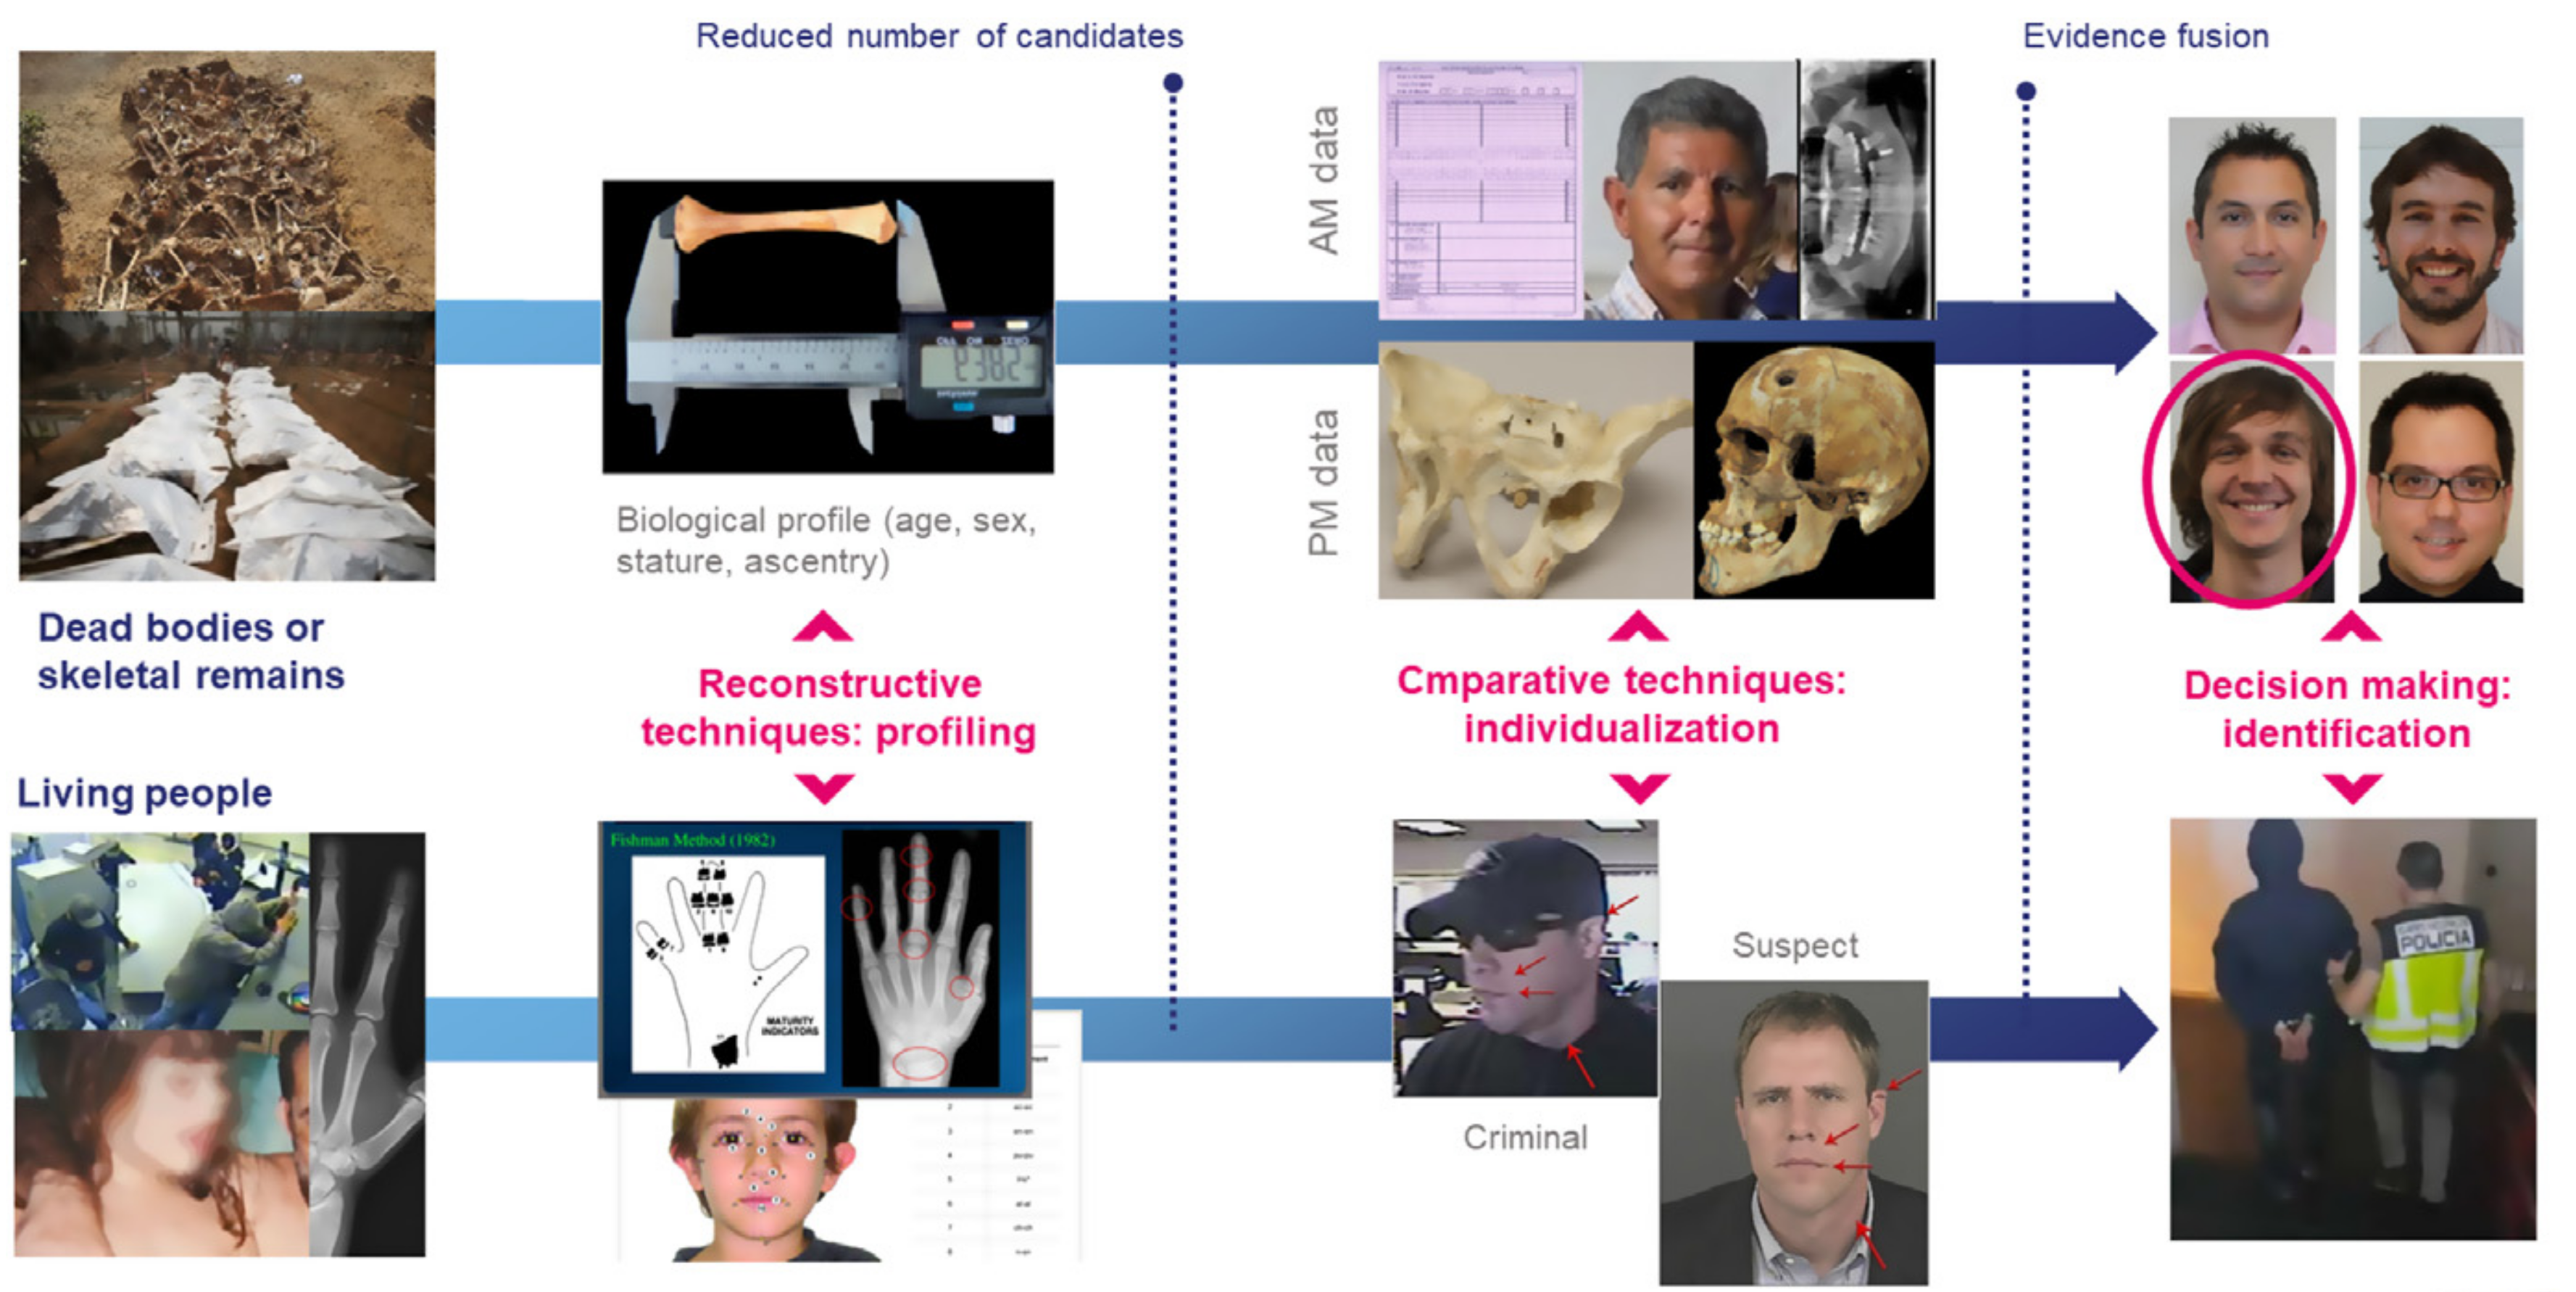
\includegraphics[width=\textwidth]{capitulos/cap_01/imagenes/SFI_pipeline.png}
    \caption{Procedimiento secuencial para la identificación forense basada en el esqueleto humano 
            (\textit{skeleton-based forensic identification}) \cite{mesejo2020}.} 
    \label{fig:SFI_pipeline}
\end{figure}

La estimación del PB en restos humanos es una tarea compleja, especialmente cuando se estima la edad en el 
momento de la muerte, ya que hay diferentes métodos a aplicar dependiendo de la fase de desarrollo del 
individuo. Las variaciones en la morfología de los huesos son bien conocidas, pero estas no siempre ocurren 
al mismo tiempo en diferentes individuos, ya que no están expuestos a las mismos condiciones genéticas y del 
entorno.

Además, como se ha mencionado anteriormente, la estimación de edad también se realiza sobre personas vivas
en casos legales donde la edad es un factor determinante \cite{schmeling2016}, por ejemplo, con menores 
migrantes no acompañados. En estos casos no se tiene acceso a los huesos de la persona de forma directa, por 
lo que el análisis se realiza sobre imágenes médicas.

% sin registros confiables, 
% en casos legales donde la edad es un factor determinante \cite{schmeling2016}. En estos casos no se tiene 
% acceso a los huesos de la persona de forma directa, por lo que el análisis se realiza sobre imágenes 
% médicas. Dependiendo de la cuestión legal, se requerirá la estimación de la edad mínima del individuo o su 
% edad más probable.

% en casos legales donde la edad es un factor determinante \cite{schmeling2016}, como en solicitudes de asilo, adopciones 
% internacionales o juicios donde se debe establecer si un individuo es menor o mayor de edad, lo que puede tener 
% consecuencias legales significativas. En estos casos no se tiene acceso a los huesos de la persona de forma 
% directa, por lo que el análisis se realiza sobre imágenes médicas. Dependiendo de la cuestión legal, se 
% requerirá la estimación de la edad mínima del individuo o su edad más probable.

% ------------------------------------------------------------------------------------------------------------
% ------------------------------------------------------------------------------------------------------------
% ------------------------------------------------------------------------------------------------------------

\section{Motivación}

Los métodos de estimación del PB se basan en la evaluación visual y en el análisis morfométrico de rasgos 
esqueléticos, que requieren de conocimiento especializado. Sin embargo, su aplicación puede presentar 
ambigüedades en su formulación que den lugar a interepretaciones variables ---muchas veces fruto de sesgos 
cognitivos \cite{nakhaeizadeh2014, cooper2019}--- y están sujetos a posibles errores de medición 
\cite{langley2018}.
Además, la gran variabilidad genética y ambiental entre individuos, que afecta la morfología del esqueleto y 
genera diferencias significativas entre poblaciones de distintas regiones \cite{ubelaker2017}, hace que muchos 
de estos métodos ---basados en muestras de referencia limitadas o no representativas de la diversidad humana 
global--- pierdan precisión. Esto puede introducir sesgos al estimar el PB de individuos de 
grupos poco estudiados o con características atípicas.

Frente a estas limitaciones, recientes avances en inteligencia artificial (IA) y machine learning (ML) han 
demostrado el potencial de mejorar la exactitud y objetividad de estimación del PB, tanto para la estimación 
de sexo \cite{curate2017, darmawan2015, pinto2016} como de edad \cite{kim2017, larson2018, lee2017}. 

Estos modelos, que emplean imágenes médicas con algoritmos de visión por computador, siguen dos principales enfoques.
En el primer enfoque, parten de un método de AF clásico e intentan automatizarlo y/o mejorarlo 
\cite{stern2014, ajafernandez2004} (véase la Figura \ref{fig:MRI_pipeline}). 
Para ello, es necesario especificar:

\begin{enumerate}

    \item cómo extraer las características relevantes de las imágenes médicas, mediante técnicas de procesamiento de 
    imágenes o morfometría tradicional; y
    
    \item un modelo de clasificación o regresión (como SVM, redes neuronales simples o árboles de decisión) 
    que opere sobre estas características predefinidas.

\end{enumerate}

\begin{figure}[h]
    \centering
    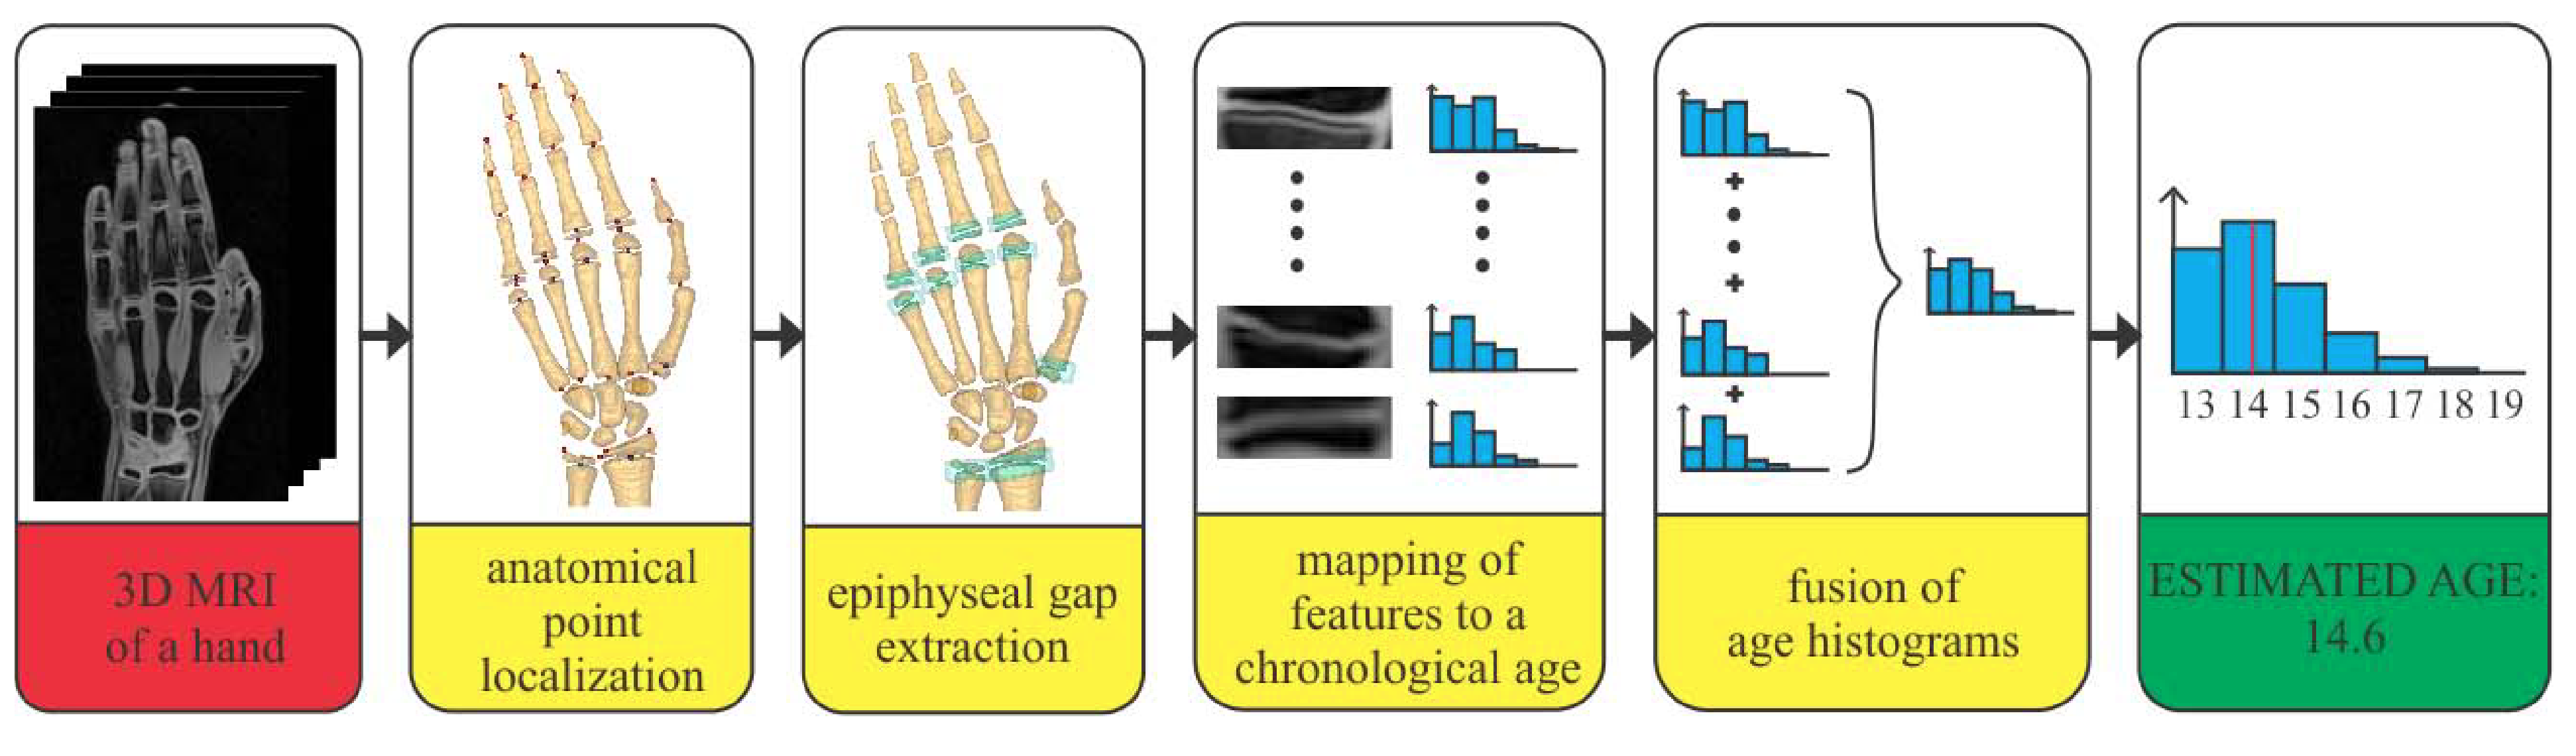
\includegraphics[width=\textwidth]{capitulos/cap_01/imagenes/MRI_pipeline.png}
    \caption{Procedimiento secuencial para el método propuesto en \cite{stern2014}.} 
    \label{fig:MRI_pipeline}
\end{figure}

En cambio, en el enfoque más popular, el \textit{end-to-end}, el modelo aprende automáticamente tanto la 
extracción de características como la clasificación/regresión a partir de los datos en bruto. Este enfoque es 
posible gracias a las redes neuronales convolucionales, que eliminan la dependencia de criterios 
antropológicos preestablecidos y permite al modelo extraer por sí mismo las características más relevantes 
para la estimación de sexo, edad, etc. 

Este enfoque se ha visto potenciado por el auge del Deep Learning, permitiendo a las CNNs aprender patrones 
complejos que podrían pasar inadvertidos por el ser humano, y mejorando la precisión de las predicciones 
\cite{stern2019, venema2022}. 
Sin embargo, aún mejorando la exactitud de las predicciones, los modelos siguen mostrando carencias respecto a 
la cuantificación de incertidumbre, pues no todas las predicciones tienen el mismo nivel de confianza o 
fiabilidad. Ya en \cite{ferrante2009} se introducía no solo la necesidad de identificar el método adecuado 
para estimar la edad a partir de los elementos disponibles, sino también de evaluar su confiabilidad y 
realizar un estudio del error arrojado por las predicciones del método. Estos generalmente se han basado en 
la estadística frecuentista \cite{verma2020, stepanovsky2024, heinrich2024}
\footnote{
    La estadística frecuentista es la corriente estadística que desarrolla a partir de los conceptos de 
    probabilidad y que se centra en el cálculo de probabilidades y el contraste de hipótesis.
}.
Un ejemplo de este tipo de análisis se ilustra en la Figura \ref{fig:regression_lentibia_stature}, donde se 
examina la distribución probabilística del error residual arrojado por el modelo de regresión propuesto en 
\cite{verma2020}.

% \begin{figure}[h]
%     \centering
%     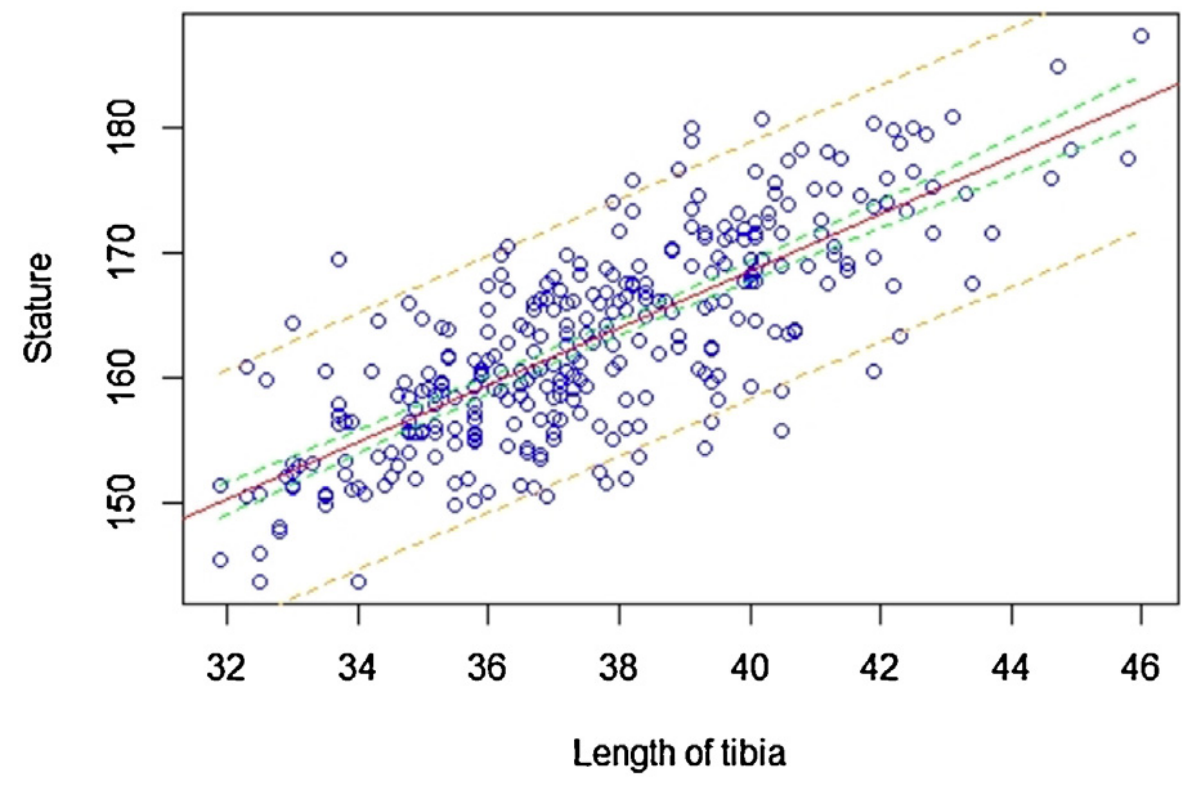
\includegraphics[width=0.7\textwidth]{capitulos/cap_01/imagenes/regression_line_lentibia_stature.png}
%     \caption[
%         Línea de regresión del modelo de regresión propuesto en \cite{verma2020} que predice la estatura
%         a partir de la longitud de la tibia.
%     ]{
%         Línea de regresión del modelo de regresión propuesto en \cite{verma2020} que predice la estatura 
%         a partir de la longitud de la tibia. En rojo, la línea de regresión; en verde, la línea de los 
%         intervalos de confianza del 95\%; y en naranja, la línea de los intervalos de predicción al 95\% de 
%         confianza.
%     } 
%     \label{fig:regression_lentibia_stature}
% \end{figure}

Aunque existen métricas para evaluar el error cuando se dispone de \textit{ground truth}, la mayoría de los 
modelos actuales se limitan a ofrecer predicciones puntuales en regresión 
\cite{park2024, imaizumi2021, stepanovsky2024} o etiquetas únicas en clasificación 
\cite{venema2022, park2024}, sin cuantificar la incertidumbre asociada a cada predicción.

Con lo anterior se expone la motivación de la aplicación de ML a la AF, así como de la necesidad de 
cuantificar la incertidumbre en las predicciones, para ofrecer garantías de confiabilidad estadística que 
aspiren a sustentar la validez legal en contextos judiciales. Algunos datos que magnifican la necesidad de 
técnicas de AF confiables actualmente son:

% 1/3 de los muertos del 11S sin identificar

\begin{itemize}

    \item En los últimos años, ha aumentado significativamente el número de cadáveres hallados en el 
    territorio español, como podemos apreciar en la Figura \ref{fig:evolucion_hallazgosID_cadaveres} 
    \cite{interior2025desaparecidos}. 
    En 2024 se ha alcanzado una cifra record, ---en gran parte debido a las inundaciones de la DANA 
    Valencia---, de 531 cadáveres en 2024, de los cuales se pudo identificar a 323.

    \begin{figure}[h]
        \centering
        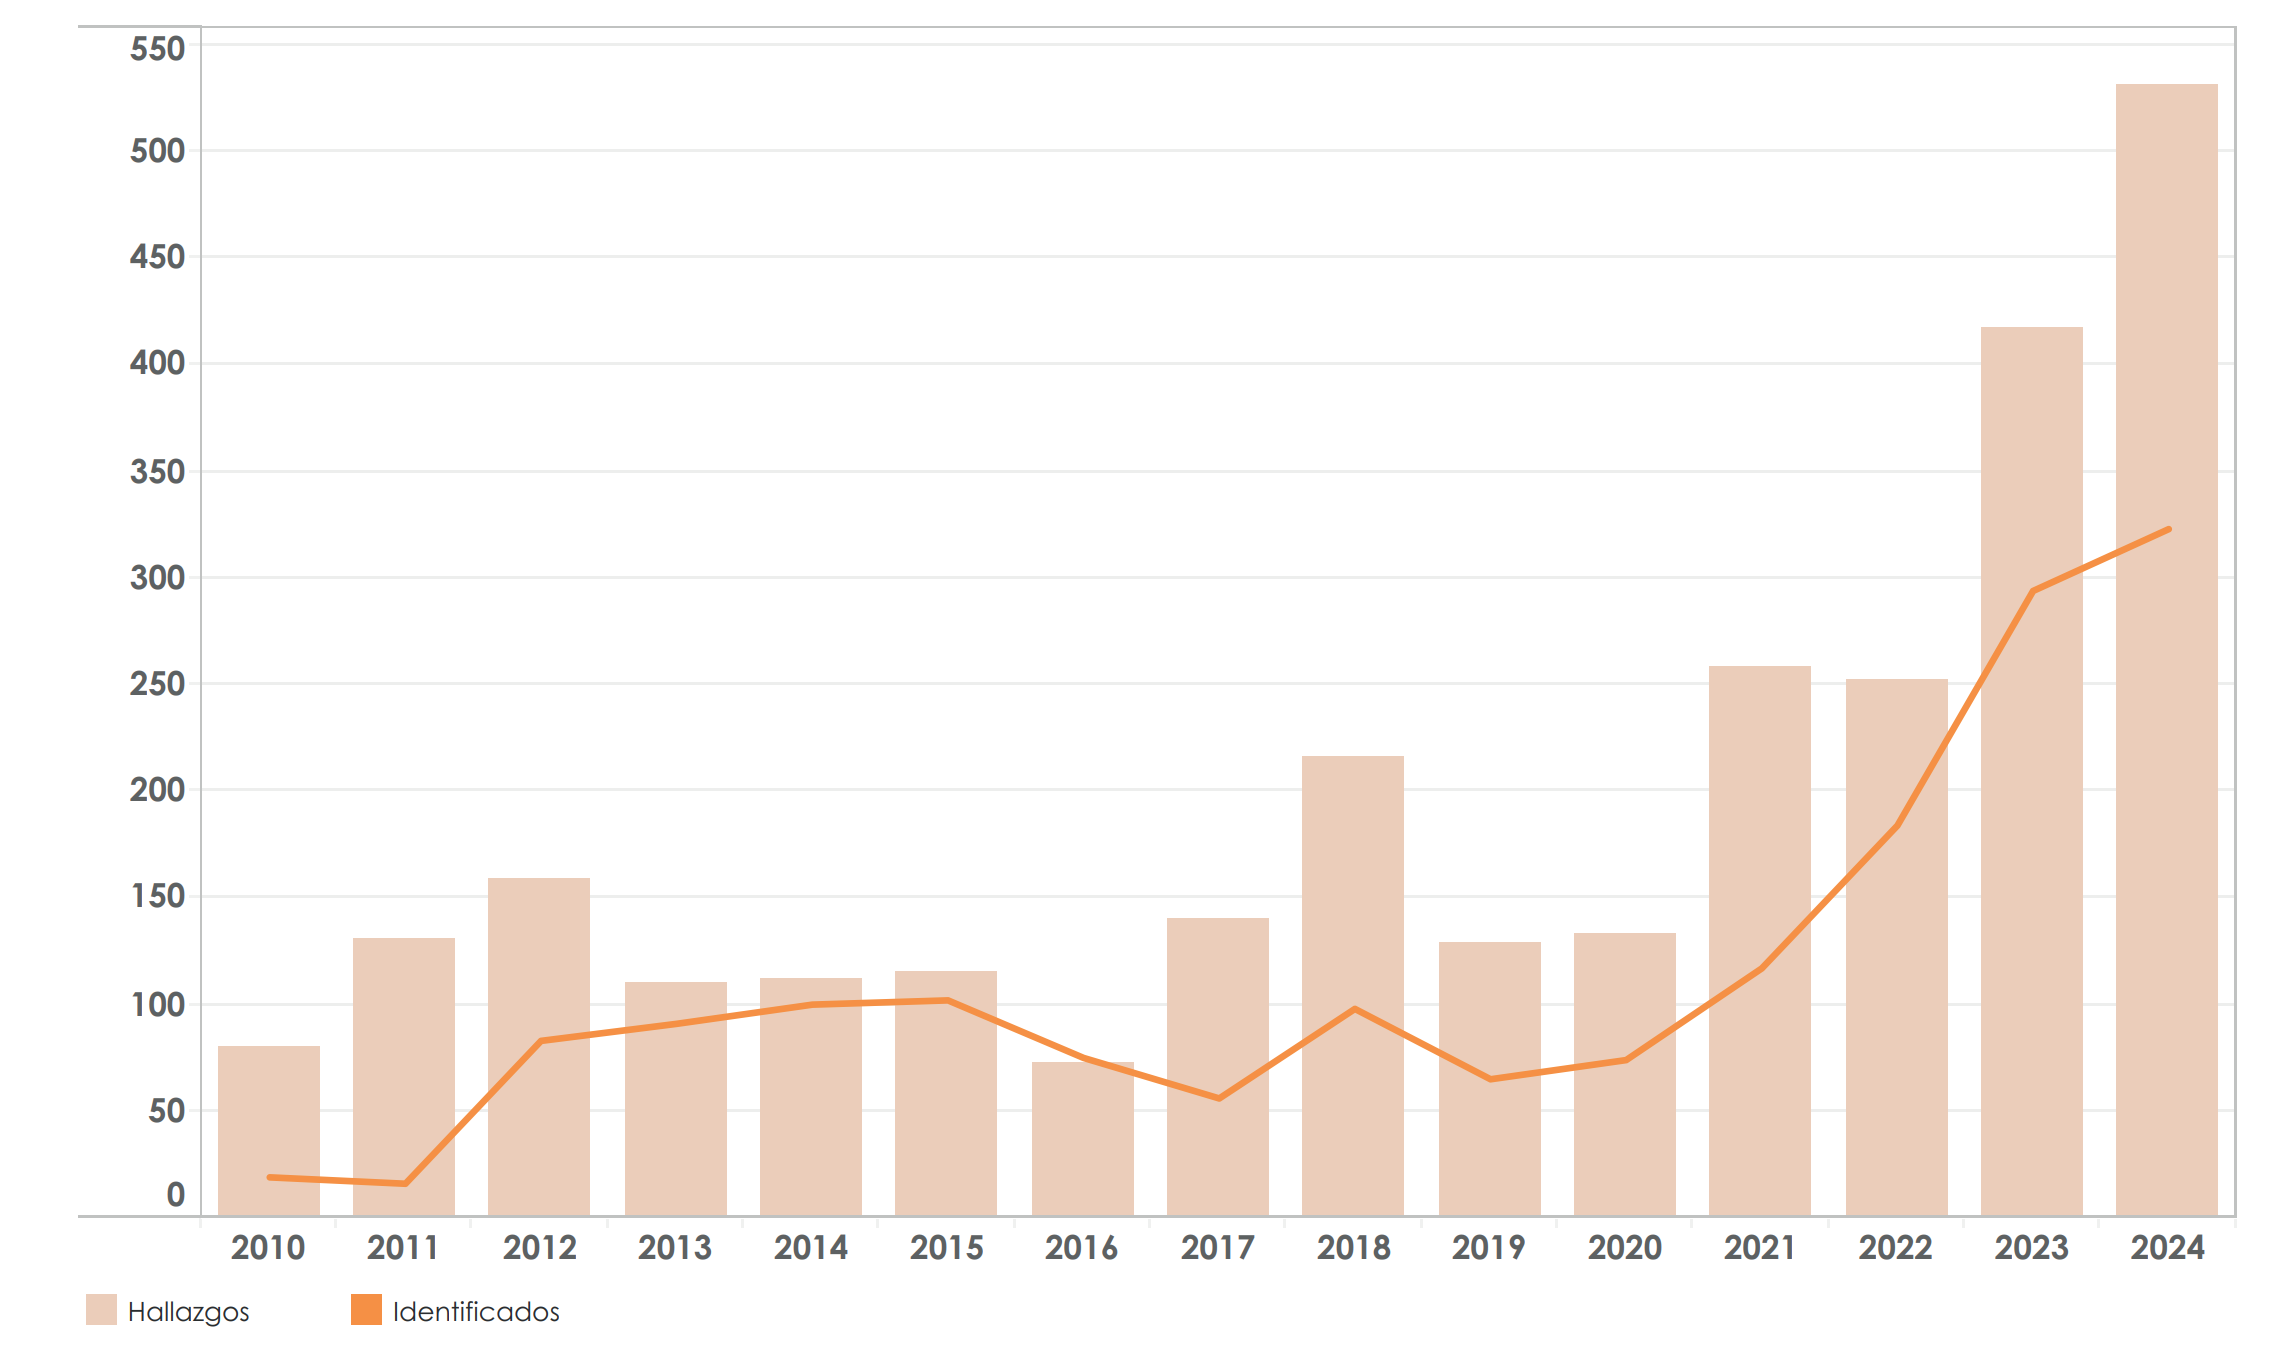
\includegraphics[width=\textwidth]{capitulos/cap_01/imagenes/hallazgos_cadaveres.png}
        \caption{
            Evolución de hallazgos/identificación de cadáveres en España (2010-2024) 
            \cite{interior2025desaparecidos}.
        } 
        \label{fig:evolucion_hallazgosID_cadaveres}
    \end{figure}

    \item En 2020, de las 2.457 fosas totales documentadas de la Guerra Civil y el franquismo, aún 1.221 
    seguían sin ser intervenidas y se estimaba que ``con una intervención oficial del Estado podrían 
    recuperarse unos 20 a 25.000 individuos'' e identificar ``entre 5 y 7.000 de ellos'', estimándose 
    necesario contar con unos 40-50 profesionales de la antropología forense \cite{etxeberria2020}. 

    % \item De acuerdo con UNICEF \cite{unicef2013}, en 2012 cerca de 230 millones de niños menores de 
    % cinco años no contaban con un registro oficial de nacimiento. Las regiones con las tasas más bajas 
    % de registro incluyen África subsahariana (44\%) y el sur de Asia (39\%). Esta situación se agrava 
    % aún más, ya que muchos niños registrados no poseen un certificado de nacimiento, y los documentos 
    % existentes suelen perderse durante procesos de migración.

    \item En España, se ha registrado en la última década (2013-2023) un aumento significativo en la llegada
    de Menores Extranjeros No Acompañados \cite{fge2024,fge2019,fge2016,fge2013}, que ha disparado 
    consigo el número de diligencias abiertas para la determinación de su edad, como se ve reflejado 
    en la Figura \ref{fig:evolucion_DPDE}.

    \begin{figure}[h]
        \centering
        \includegraphics[width=\textwidth]{capitulos/cap_01/imagenes/dpde_España.png}
        \caption{
            Evolución del número de diligencias preprocesales de determinación de edad abiertas en 
            España (2011–2023). 
            Elaboración propia a partir de \cite{fge2013,fge2016,fge2019, fge2024}.
        } 
        \label{fig:evolucion_DPDE}
    \end{figure}

    \item La relevancia de la ciencia forense en la identificación de víctimas y la protección de la dignidad 
    humana ha convertido su aplicación en un pilar fundamental de los derechos humanos y la justicia 
    internacional, naciendo así la  \textbf{acción forense humanitaria} \cite{cordner2017}. Esta disciplina 
    emplea la ciencia forense con un propósito exclusivamente humanitario, con los objetivos de: identificar 
    a las personas fallecidas, gestionar dignamente sus restos y aliviar el sufrimiento de sus familias en 
    situaciones de conflicto, migración y desastres naturales \cite{tidballbinz2021}. 

\end{itemize}

% ------------------------------------------------------------------------------------------------------------

\section{Objetivos}

La \textbf{\textit{Conformal Prediction}} emerge como un marco teórico robusto para generar intervalos de 
predicción con garantías estadísticas sólidas, independientemente de la distribución subyacente de los datos. 
A diferencia de los enfoques tradicionales, este método no solo ofrece predicciones puntuales, sino que 
cuantifica la incertidumbre asociada a cada estimación mediante intervalos adaptativos o conjuntos de 
predicción que reflejan la confiabilidad de la predicción en cada caso particular.

% A revisar próximo párrafo: ¿se usarán finalmente datos tabulares?

Este proyecto tiene un doble objetivo: por un lado, desde un prisma teórico, estudiar las ventajas y costes 
asociados a las diversas técnicas de inferencia conformal actuales
\todo{
    ¿Es más correcto ``técnicas de cuantificación de la incertidumbre''?
}
; y, por otro, aplicarlo a un contexto práctico como es es el problema de estimación del PB, 
centrándonos en la estimación de edad y de sexo a partir de datos biológicos e imágenes médicas. De esta 
forma, cuando estemos ante datos biológicos ambiguos, la conformal prediction podrá devolver conjuntos de 
predicciones con más de una etiqueta predicha (p.ej., \{masculino, femenino\}) en problemas de clasificación, 
o intervalos de predicción más amplios (p.ej., edad$\in$[17,20]) en problemas de regresión, en ambos casos 
para un nivel de confianza determinado.

Por tanto, ponemos desgranar los objetivos en:

\begin{itemize}

    \item Estudiar de forma exhaustiva la bibliografía sobre \textit{conformal prediction} y sus diversas 
    variantes, así como de la estimación de sexo y edad, centrando nuestra atención en el estado del arte.

    \item Implementar, entrenar y validar modelos de regresión ---en problemas de estimación de edad--- y 
    clasificación ---tanto en problema de estimación de sexo como edad legal--- a los que aplicar la 
    inferencia conformal.

    \item Comparar los intervalos y conjuntos de predicciones generados para evaluar su calibración empírica, 
    robustez ante datos ambiguos y utilidad forense, contrastándolos con métodos tradicionales (p.ej., 
    intervalos de confianza clásicos).  

    \item Realiza una primera aproximación a un marco interpretable y con garantías estadísticas para la 
    estimación del perfil biológico, donde la incertidumbre cuantificada pueda integrarse en informes 
    periciales bajo estándares jurídicos.

\end{itemize}

En resumen, este trabajo pretende explorar la integración de marcos probabilísticos en la práctica forense
que capturen la incertidumbre de los problemas, y facilitar el uso de la inferencia conformal en ellos. 
Este enfoque proporciona estimaciones calibradas de incertidumbre, con garantías estadísticas de cobertura 
válidas bajo supuestos mínimos, útiles para la toma de decisiones fundamentadas en contextos prácticos 
donde la interpretabilidad y robustez son críticas.

% ------------------------------------------------------------------------------------------------------------

\section{Planificación económica y temporal del proyecto}

\todo{Falta escribir este apartado}



